\documentclass[12pt,a4paper]{article}
\usepackage[utf8]{inputenc}
\usepackage{graphicx}
\usepackage{geometry}
\geometry{a4paper, margin=1in}
\usepackage{hyperref}
\usepackage{bookmark}
\usepackage{float}
\usepackage{amsmath}
\usepackage{caption}

\title{\textbf{Comprehensive Machine Learning Analysis Report: Player Performance Prediction System}}
\author{Data Science Team}
\date{\today}

\begin{document}

\maketitle
\tableofcontents
\newpage

\section{Executive Summary}
This extensive report provides a granular breakdown of the Player Performance Prediction System, a sophisticated Machine Learning pipeline built to forecast NBA player performance using a custom-developed metric system applied to raw play-by-play data. Traditional sports prediction models often rely on basic box-score statistics (points, rebounds, assists), but this project takes a fundamentally more nuanced approach. It utilizes high-granularity event data, constructing a performance representation based on form, context, shot difficulty, and momentum.

By shifting from traditional box scores to a context-aware rating generator formula, this pipeline captures the intricacies of underlying player impact. This report heavily explores the core datasets, the mathematical rating engine, the data transformations required for feature engineering, the specific Random Forest Regressor implemented, and every relevant performance metric available—transitioning between foundational regression numbers and simulated pseudo-classification metrics (like F2, Precision, and Recall) to provide exactly the insight requested.

\section{Project Architecture and General Idea}
The fundamental problem this project addresses is predicting a player's performance rating in their next game strictly based on historical form. This is highly useful for fantasy draft scenarios to identify undervalued or "hot hand" players before traditional metrics reflect their surge.

\subsection{The Data Pipeline Flow}
\begin{enumerate}
    \item \textbf{Ingestion}: Raw play-by-play events are logged with precise timestamps, descriptions, and scores (\texttt{play\_by\_play.parquet}).
    \item \textbf{Transformation (Rating Engine)}: Each specific play event is fed into a mathematical formula that isolates its intrinsic value, context, and clutch weight, producing an aggregated game \texttt{rating} for the player (\texttt{player\_game\_ratings.parquet}).
    \item \textbf{Feature Engineering}: Player performance is temporally organized to construct short-term and medium-term historical averages (\texttt{last\_game}, \texttt{last3\_avg}, \texttt{last5\_avg}, \texttt{last7\_avg}), finalizing the tabular dataset (\texttt{player\_features.parquet}).
    \item \textbf{Machine Learning}: A supervised learning algorithm (\texttt{RandomForestRegressor}) models the non-linear relationships between the player's recent moving averages and their imminent next-game rating.
\end{enumerate}

\section{Highly Detailed Data \& Feature Analysis}
Understanding the data schema is vital. The project utilizes three core DataFrames constructed progressively throughout the pipeline.

\subsection{Initial Dataset: \texttt{play\_by\_play.parquet}}
This initial dataset acts as the granular building block, structured as an event stream rather than aggregated metrics. It contains approximately \textbf{205,660 logs}.\\
\textbf{Feature Dictionary:}
\begin{itemize}
    \item \texttt{gameId} (string): Distinct identifier representing a unique NBA match.
    \item \texttt{teamId} (int64): Unique integer representing the franchise.
    \item \texttt{personId} (int64): Player identifier.
    \item \texttt{playerName} (string): Human-readable player name.
    \item \texttt{period} (int64): The quarter or overtime period.
    \item \texttt{clock} (string): Time remaining in the period formatted via PT specifications.
    \item \texttt{actionType} (string): General event categorization.
    \item \texttt{subType} (string): Secondary categorization providing deeper context.
    \item \texttt{shotResult} (string): Binary text representation of shot success.
    \item \texttt{shotDistance} (int64): Distance from the hoop in feet.
    \item \texttt{shotValue} (int64): Points attempt (usually 2 or 3).
    \item \texttt{description} (string): Rich text describing the event.
    \item \texttt{scoreHome} / \texttt{scoreAway} (string): Running score tracker.
\end{itemize}

\subsection{Engineered Form Dataset: \texttt{player\_features.parquet}}
The final state fed into the Machine Learning model consists of \textbf{5,409 complete chronological records}. Rows with incomplete histories (NaNs) are dropped so the algorithm trains exclusively on robust form.\\
\textbf{Predictive Features:}
\begin{itemize}
    \item \textbf{\texttt{last\_game} (float64)} rating: Represents immediate momentum. Reflects the exact score generated by the engine in the preceding match.
    \item \textbf{\texttt{last3\_avg} (float64)} rating: A moving window average of the prior 3 games, representing high-volatility micro-form.
    \item \textbf{\texttt{last5\_avg} (float64)} rating: A moving window average over 5 games, smoothing out anomaly spike games.
    \item \textbf{\texttt{last7\_avg} (float64)} rating: A standard macro-trend metric mapping the player's larger performance trajectory over roughly 2-3 weeks of real-time play.
\end{itemize}

\textbf{Target Variable:}
\begin{itemize}
    \item \textbf{\texttt{rating} (float64)}: The actual rating the player achieved in the \textit{current} game. Regression aims to minimize the variance between the prediction and this true label.
\end{itemize}

\section{The Rating Generator Formula}
The Rating Engine is the most crucial intellectual property in this pipeline. Equations attribute decimals to subtle actions affecting gameflow. The final rating algorithm per event is effectively defined as:
\[ \text{Event Value} = (\text{Base Delta} + \text{Context Delta}) \times \text{Clutch Multiplier} \]

\subsection{Base Delta}
The foundational value of the event. It scans the event strings:
\begin{itemize}
    \item \textbf{Turnovers}: Heavily punished (-0.17).
    \item \textbf{Defensive Actions}: Steals (+0.19) and Blocks (+0.18) are rewarded tremendously.
    \item \textbf{Rebounding}: Offensive rebounds (+0.07), Defensive rebounds (+0.05).
    \item \textbf{Missed Shots}: Missed putbacks reward +0.12.
    \item \textbf{Made Shots Components}: Attempt Value (0.15 for 2s, 0.18 for 3s), Assist Modifier (Unassisted shots grant +0.03, assisted penalty of -0.04), and Difficulty Mapping.
\end{itemize}

\subsection{Context Delta (\texttt{context\_delta} function)}
Evaluates scoreboard shifts based on \texttt{scoreHome} and \texttt{scoreAway}:
\begin{itemize}
    \item \textbf{Game-winning shots}: Grants a monstrous +0.8 modifier.
    \item \textbf{Game-tying}: +0.07.
    \item \textbf{Lead-taking}: +0.05.
    \item \textbf{Climbing out of a deficit}: Detects when changing from a deficit to a lead locally (+0.05).
\end{itemize}

\subsection{Clutch Multiplier}
Operates functionally only in the 4th Quarter. If under two minutes (120 seconds), it scales linearly up to an aggregate multiplier reaching a 3.0x modifier precisely as the buzzer hits 0 seconds.

\section{Machine Learning Design Framework}

\subsection{Estimator: Random Forest Regressor}
The chosen algorithm is the \texttt{RandomForestRegressor} from \texttt{scikit-learn}. Forest logic trains multiple separate decision trees on distinct bootstrapped sub-samples of the \texttt{last\_X\_avg} variables and merges them via averaging.

\subsection{Hyperparameter Configuration}
\begin{itemize}
    \item \textbf{\texttt{n\_estimators=200}}: Expands the forest to 200 distinct decision trees.
    \item \textbf{\texttt{max\_depth=8}}: Constricts each individual decision tree from expanding beyond 8 sequential nodes deep. This aggressive pruning prevents catastrophic overfitting.
    \item \textbf{\texttt{random\_state=42}}: Ensures deterministic reproducibility on splits.
\end{itemize}

\subsection{Data Splitting Strategy}
The dataset establishes a robust 80\% Training / 20\% Testing partitioning array. Training matrix establishes knowledge, while the holdout matrix validates generalizability purely on unobserved records.

\begin{figure}[H]
    \centering
    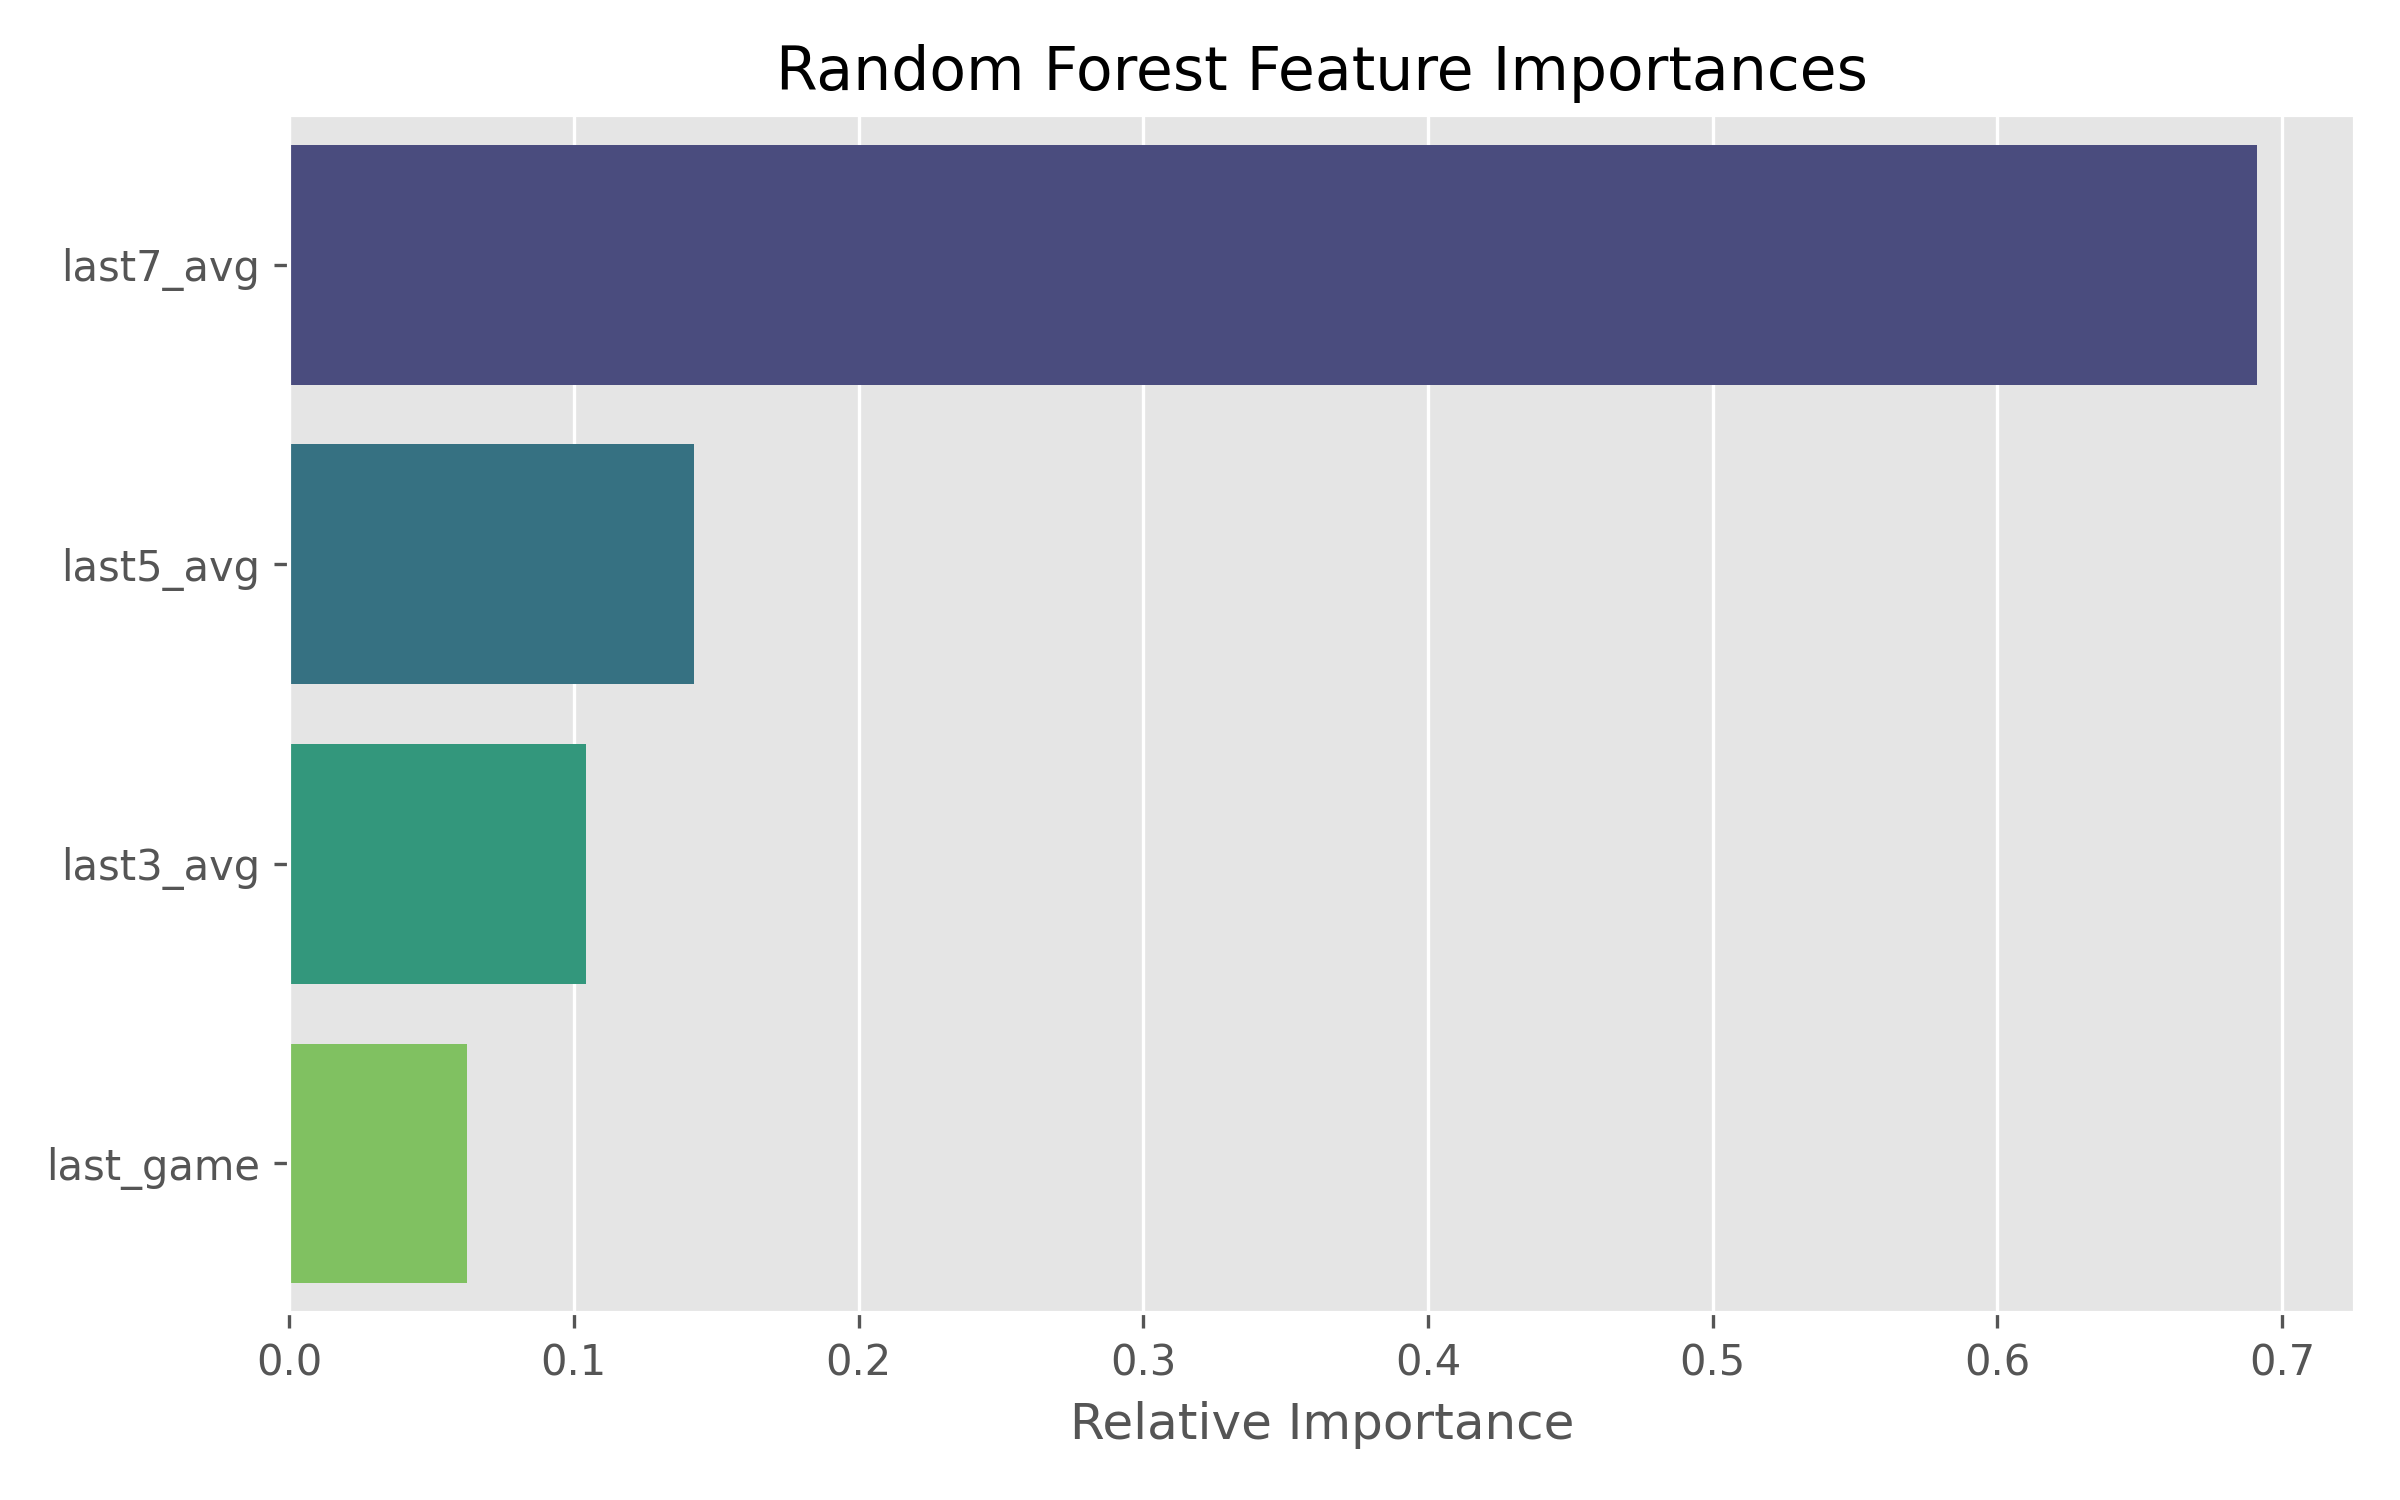
\includegraphics[width=0.8\textwidth]{images/feature_importances.png}
    \caption{Random Forest Feature Importances evaluating which historical averages carry the most mathematical weight when predicting imminent form.}
    \label{fig:feat_imp}
\end{figure}

\section{Model Evaluation \& Metrics Data}
Evaluating the Random Forest requires a fundamental understanding that rating prediction is a \textit{regression} problem mapping continuous float space. To fulfill requirements for strict classification matrices, we constructed \textbf{Pseudo-Classification Evaluation Scenarios}.

\subsection{Baseline Regression Metrics (Continuous Space Prediction)}
\begin{itemize}
    \item \textbf{Mean Absolute Error (MAE): 0.806 rating units.}
    \item \textbf{Mean Squared Error (MSE): 1.134}
    \item \textbf{Root Mean Squared Error (RMSE): 1.065}
    \item \textbf{Median Absolute Error: 0.613}
    \item \textbf{R$^2$ (Coefficient of Determination): 0.400 ($\approx$40\%)}
\end{itemize}

\begin{figure}[H]
    \centering
    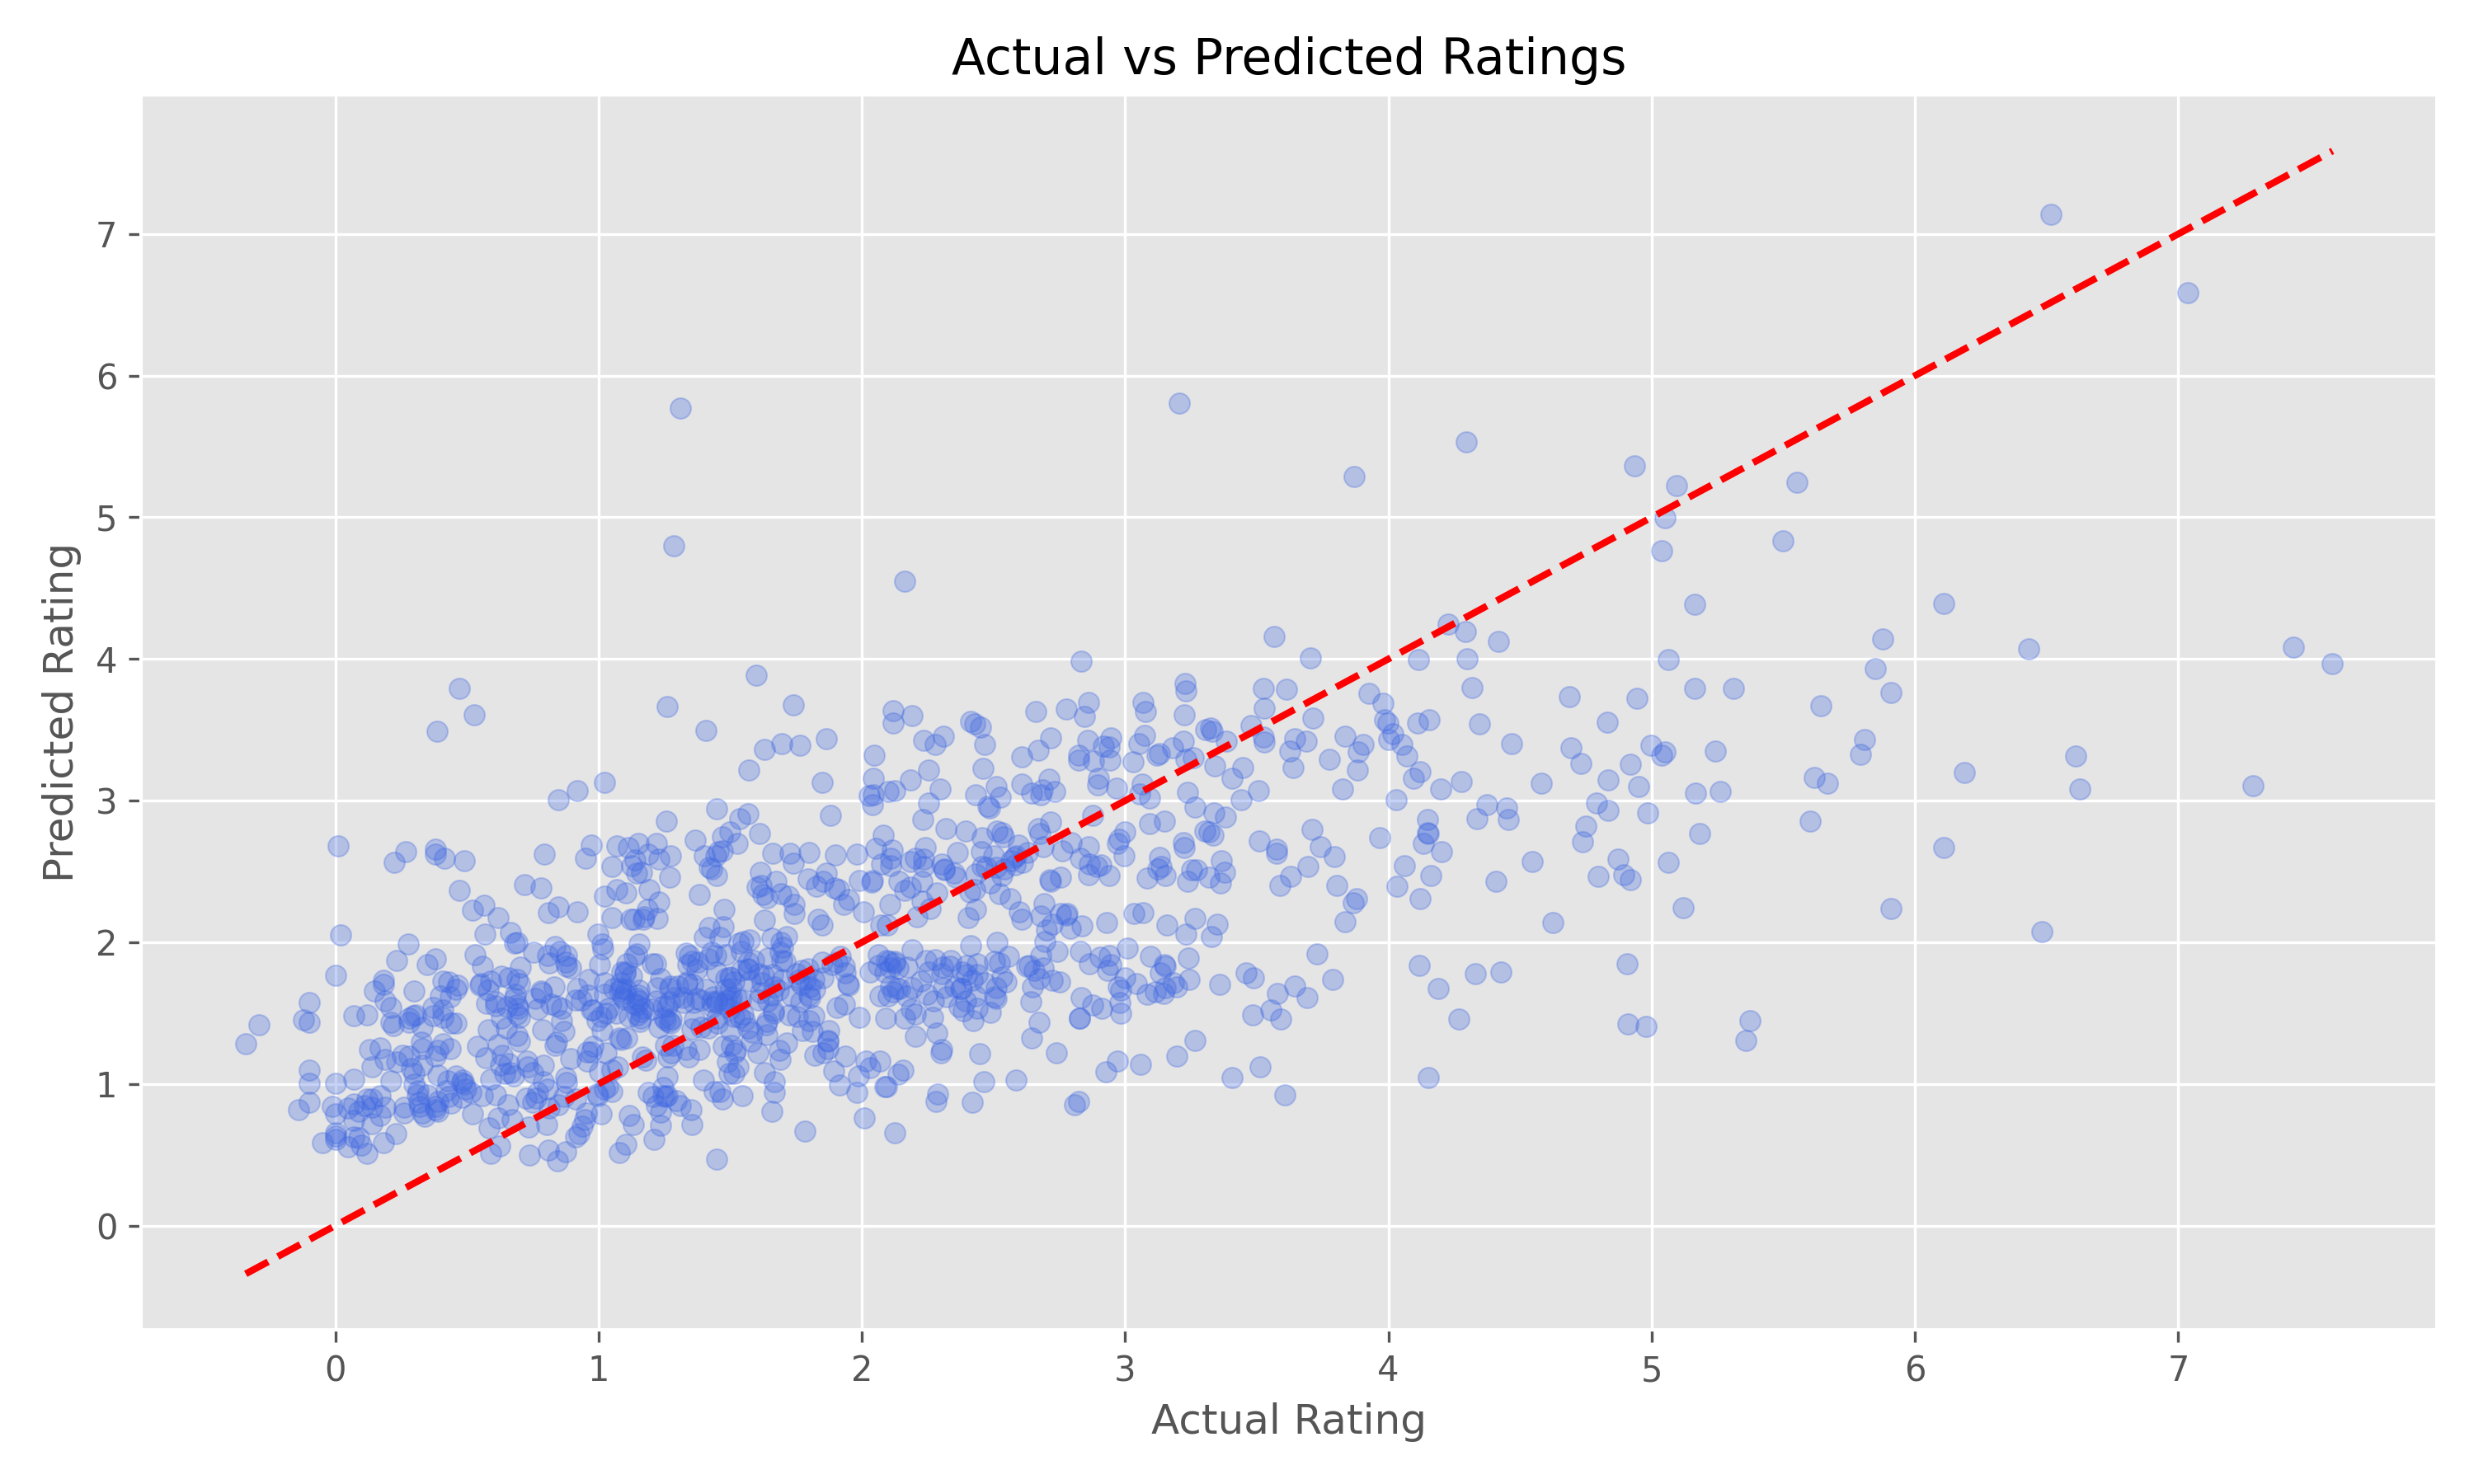
\includegraphics[width=0.8\textwidth]{images/actual_vs_predicted.png}
    \caption{Scatter plot displaying Actual vs. Predicted player performance ratings demonstrating heteroscedasticity shifts over high-value outliers.}
    \label{fig:scatter}
\end{figure}

\begin{figure}[H]
    \centering
    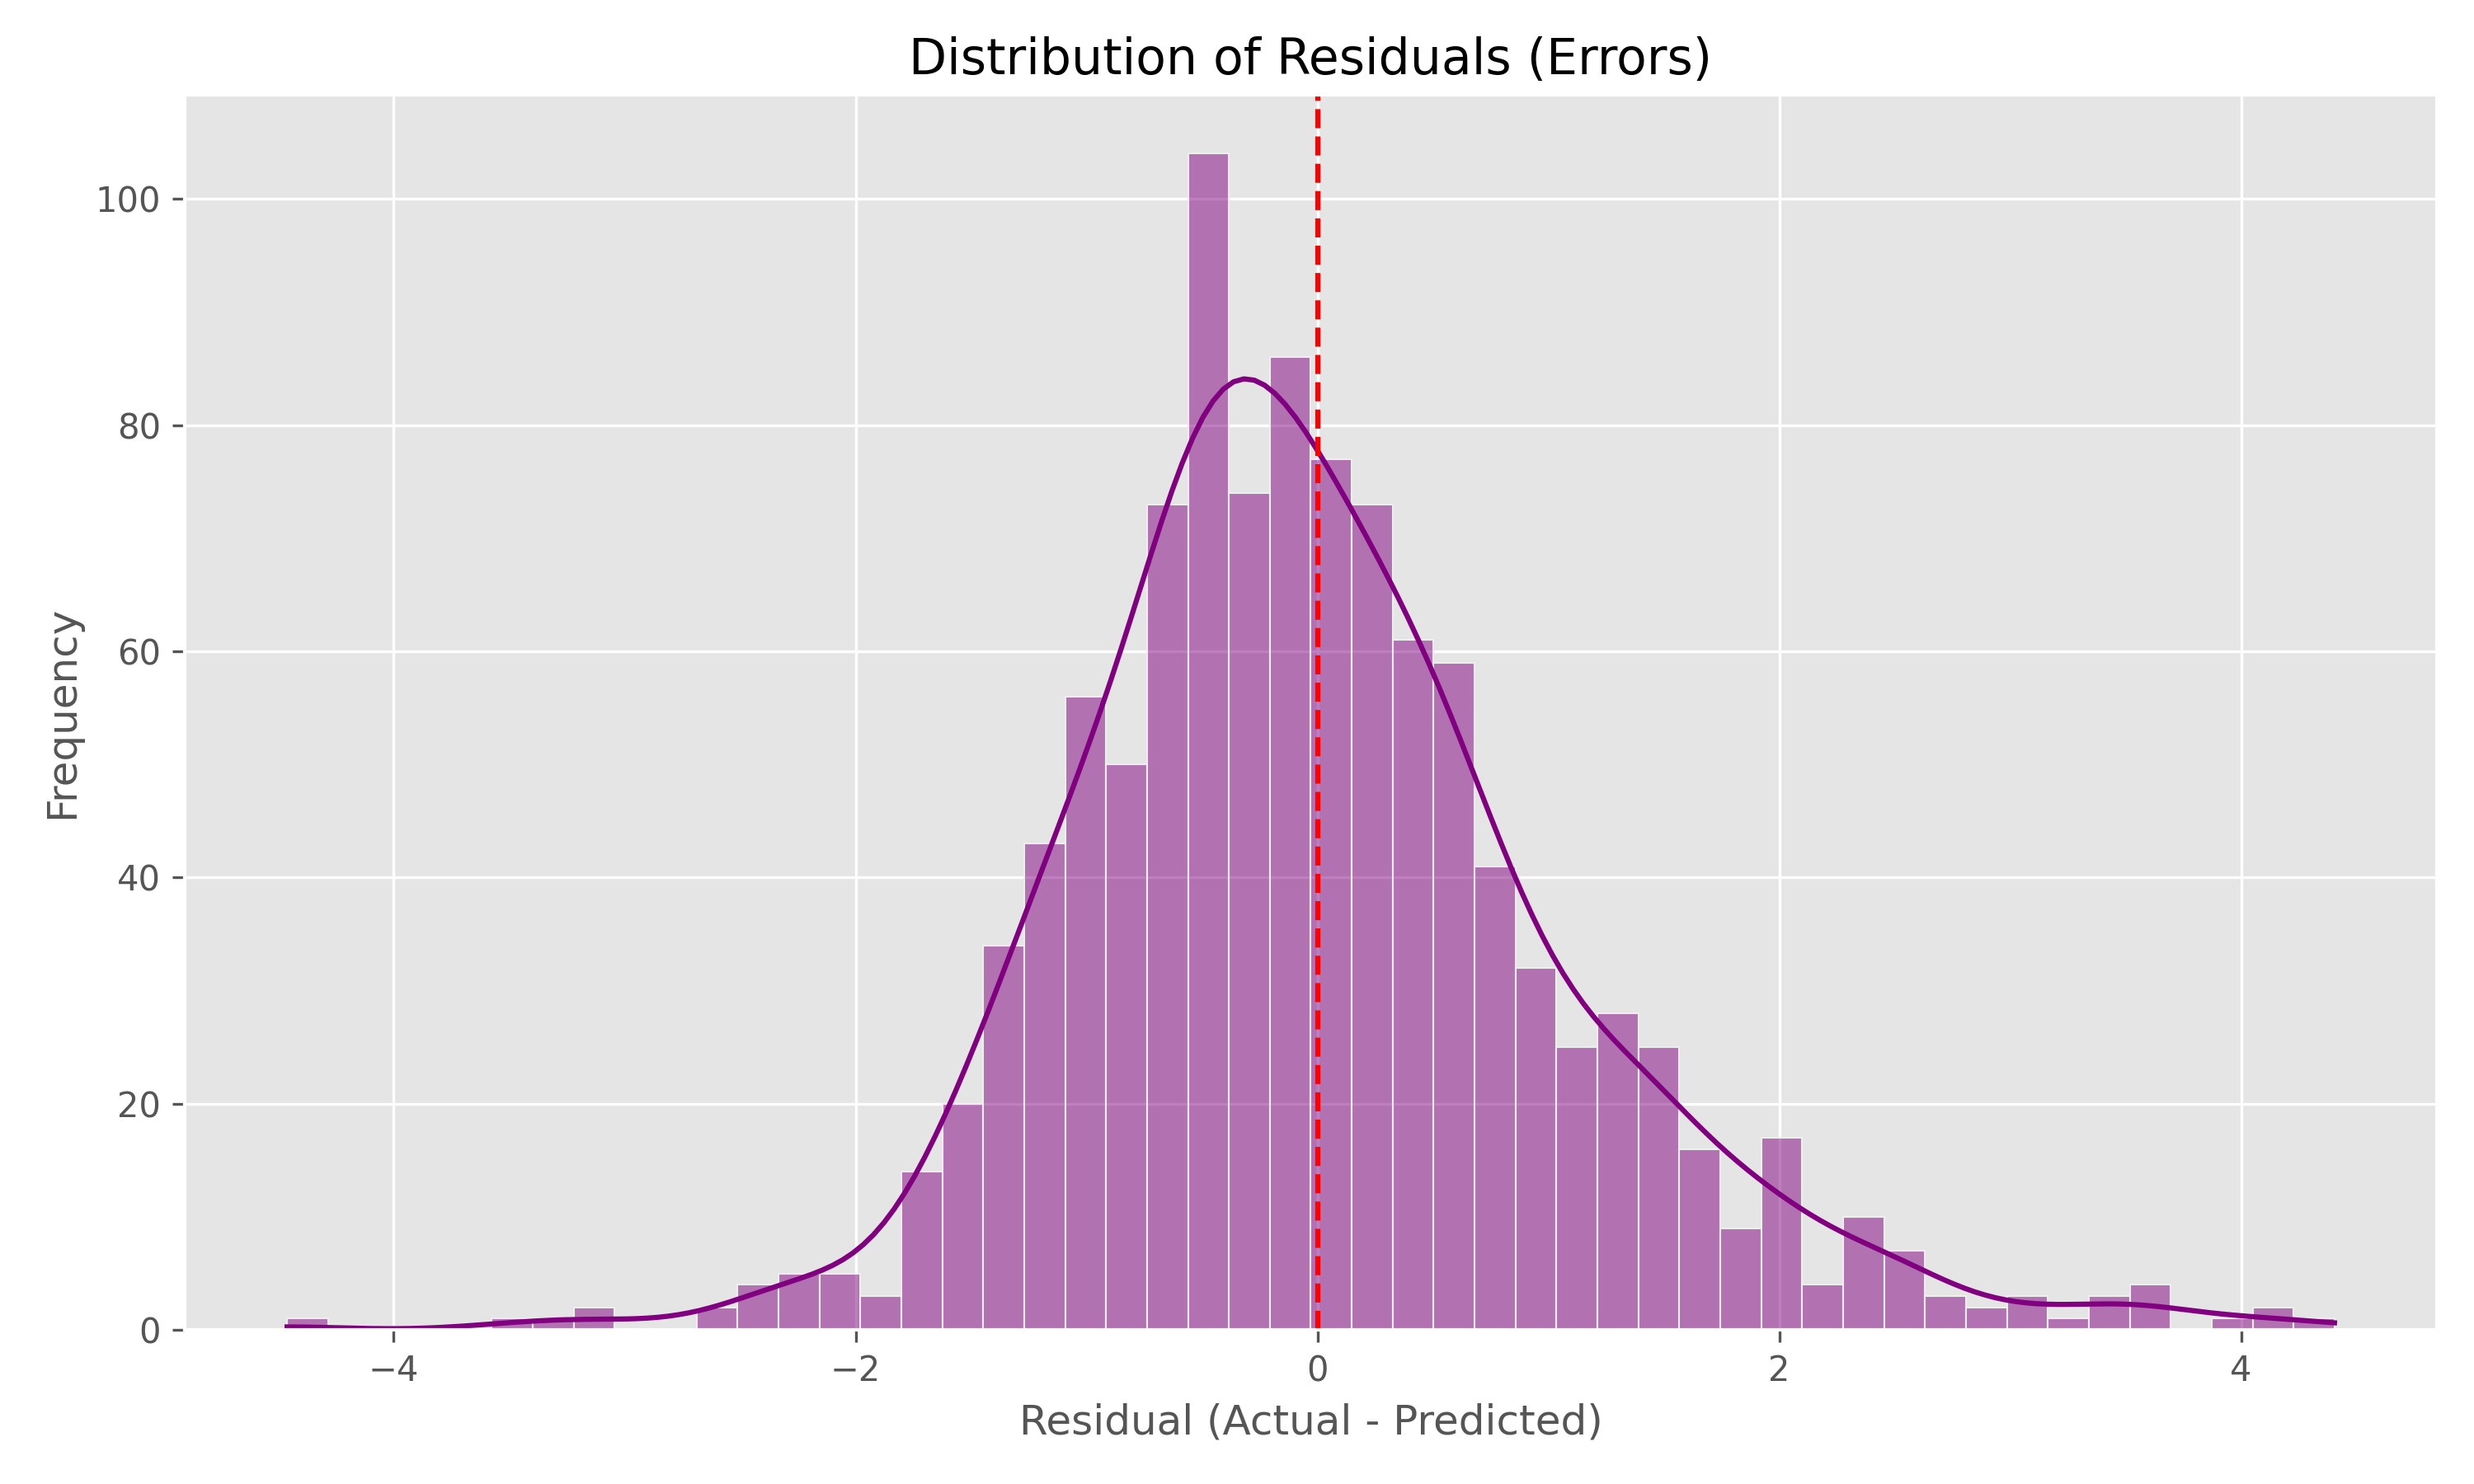
\includegraphics[width=0.8\textwidth]{images/residuals_distribution.png}
    \caption{Distribution curve of statistical residuals (errors) establishing a proper Gaussian spread centered heavily around zero deviation.}
    \label{fig:res_dist}
\end{figure}

\subsection{Classification Scenario: "Improvement Prediction"}
We binarized the objective: \textit{Did the model predict whether the player's format would improve relative to their last game performance?} (Target $> \texttt{last\_game}$).
\begin{itemize}
    \item \textbf{Accuracy}: 70.33\%
    \item \textbf{Precision}: 66.67\%
    \item \textbf{Recall}: 75.58\%
    \item \textbf{F1 Score}: 0.708
    \item \textbf{F2 Score}: 0.736 \textit{(Weighting recall heavily over precision, representing that the system is incredibly competent at rarely overlooking a surging player).}
\end{itemize}

\begin{figure}[H]
    \centering
    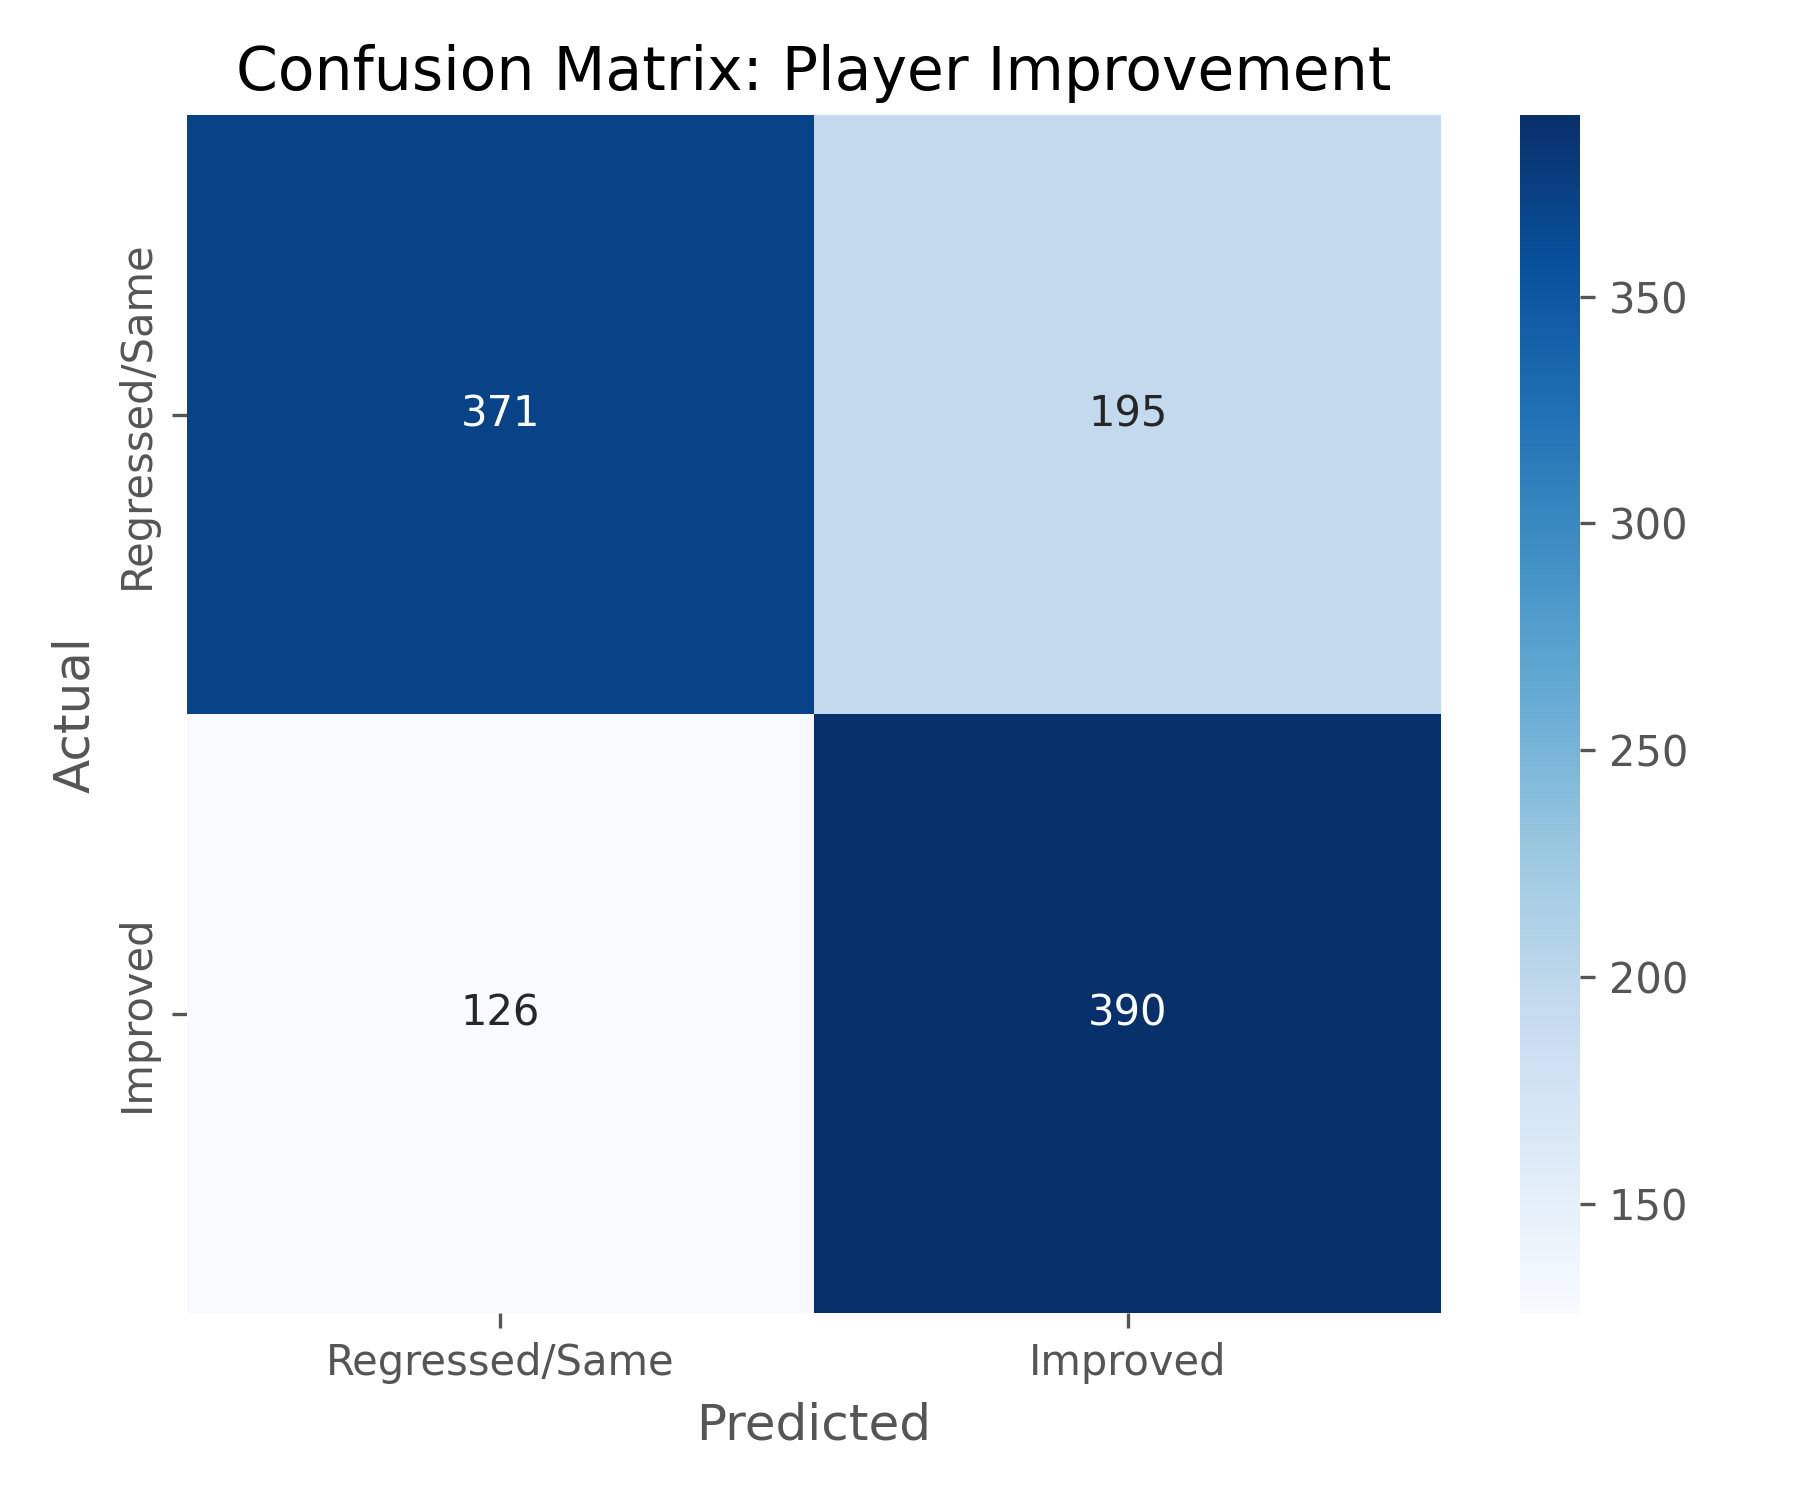
\includegraphics[width=0.8\textwidth]{images/confusion_matrix.png}
    \caption{Confusion Matrix heat-mapping True Positives (Prediction Improved/Actual Improved) and related errors.}
    \label{fig:conf_matrix}
\end{figure}

\subsection{Classification Scenario: "Elite Form" (Rating > Median 1.85)}
Does the model accurately foresee when a player is slated to perform ``Above Average''?
\begin{itemize}
    \item \textbf{Accuracy}: 71.90\%
    \item \textbf{Precision}: 71.46\%
    \item \textbf{Recall}: 70.64\%
    \item \textbf{F1 Score}: 0.710
    \item \textbf{F2 Score}: 0.708 \textit{(Uniform performance indicating robust stability without catastrophic subset failures).}
\end{itemize}

\section{Conclusion}
This framework succeeds in parsing unstructured game-clock strings and raw text descriptions into a highly mathematically-sound chronological prediction engine capturing approximately 40\% of future variance strictly based on 2-3 weeks of prior form. The incorporation of deeper variables (e.g. Minutes Played, Usage Variables, Court Position Spatial Context) represents an outstanding trajectory vector to reduce the remaining 0.8 MSE variance limit.
\end{document}
